\section{Introducción}

Existe una gran variedad de problemas que pueden ser modelados por medio de sistemas de equaciones lineales. Estas ecuaciones pueden ser expresadas mediante un sistema matricial que se puede escribir de la forma $Ax = b$ donde $A \in \mathbb{R}^{n \times n}$ y $x,b \in \mathbb{R}^{n \times 1}$. Una vez representado, se debe buscar alguna forma de resolver el sistema, es decir, buscar el vector $x$. Existen numerosas maneras de resolver este problema, entre ellas tenemos por ejemplo el clásico algoritmo de eliminación gaussiana y la factorización LU.

El objetivo de este trabajo práctico es modelar y resolver el problema de la difusión del calor en la pared de un horno circular. A priori, lo que sabemos es que el calor se propaga siguiendo la ecuación diferencial dada por el laplaciano en función del ángulo y la distancia desde el centro del horno. Aunque esta ecuación diferencial tiene una solución analítica, el trabajo practico apunta a que modelemos este problema discretizando el dominio en coordenadas polares y planteando el sistema de ecuaciones dado por el laplaciano de forma matricial. De esta forma podemos encontrar una aproximación de la temperatura en cada punto de la discretización.

Por cuestiones de seguridad e integridad estructural del horno, la isoterma 500$^{\circ}$C (una curva inducida por la temperatura interna y externa, y en donde la temperatura es efectivamente de 500$^{\circ}$C) deberá hallarse en el rango definido entre el radio interno y externo de la pared. Por esta razón, una vez calculada la temperatura aproximada en diferentes puntos de la discretización, tendremos como objetivo encontrar de alguna forma ésta isoterma, y asi comprobar la estabilidad del horno. Para ello propondremos diferentes algoritmos que aprovechen dicha discretización para aproximar la ubicación de la misma. Estas problemáticas pueden verse claramente en las siguientes figuras:

\begin{figure}[h]
  \centering
  \begin{minipage}[b]{0.35\textwidth}
    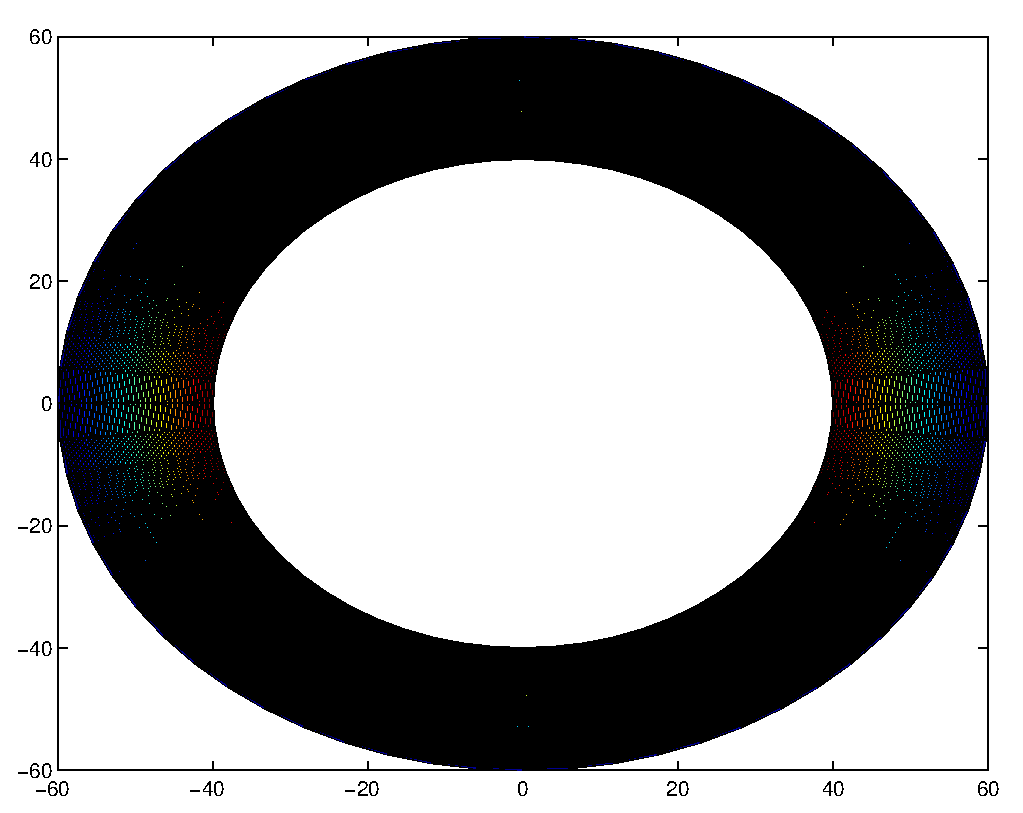
\includegraphics[width=\textwidth]{graficos/isotermaIdeal_heat.eps}
    \caption{Heat map.}
  \end{minipage}
  \hspace{1cm}
  \begin{minipage}[b]{0.30\textwidth}
    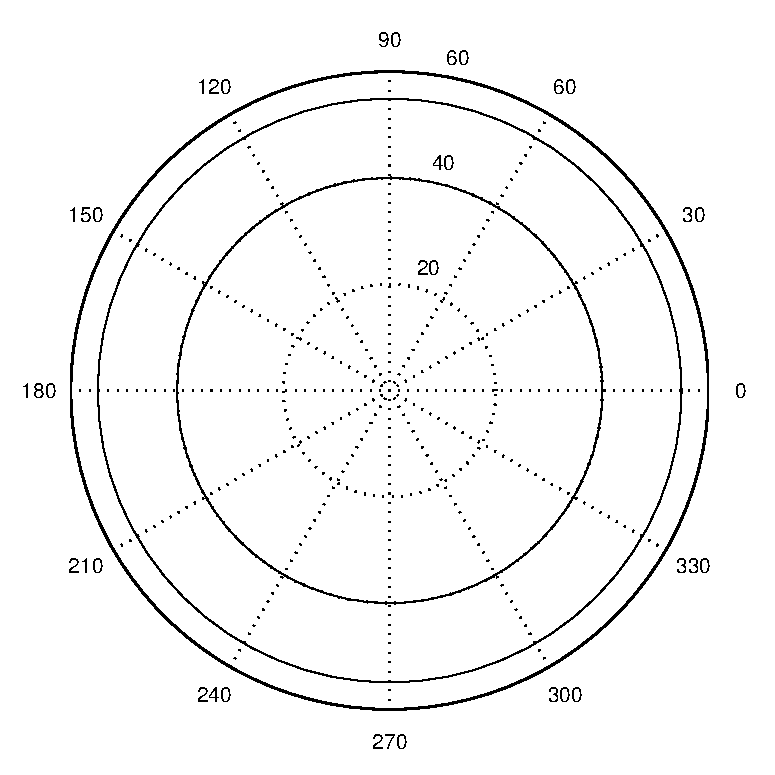
\includegraphics[width=\textwidth]{graficos/isotermaIdeal.eps}
    \caption{Isoterma.}
  \end{minipage}
\end{figure}

En el heat map se puede ver como la temperatura representada con colores va bajando a medida que uno se aleja de la pared interna del horno. A su vez, en el gráfico de la isoterma podemos ver la pared interna del horno y la isoterma 500$^{\circ}$C. En este caso, dado que no toca la pared externa del horno decimos que el mismo es estable. Notar que las isotermas no necesariamente son circulares, dado que la temperatura externa puede variar dependiendo del angulo. Este es simplemente un ejemplo ilustrativo.

En un primer momento, implementaremos y experimentaremos con el método de eliminación gausiana y la factorización LU. Evaluaremos que método es mejor dependiendo de las diferentes condiciones del horno y del grado de granularidad. A su vez analizaremos que método se comporta mejor al tener condiciones de temperatura variables, como por ejemplo en el caso en el que el vector de variables independientes $b_t$ varie con el tiempo. A priori, sabemos que para una única instancia la eliminación gaussiana y la factorización LU pertenecen a \order{n^3}. Esto se debe a que la eliminación gaussiana simplemente transforma el sistema original en uno equivalente que es triangular superior en \order{n^3}, en donde n es el numero de incógnitas. Luego se resuelve este sistema en \order{n^2}. Por otro lado, la factorizacion LU transforma el sistema original en un sistema del tipo $LUx = b$, donde L es una matriz triangular inferior y U es una matriz triangular superior en costo \order{n^3}. Finalmente, se resuelven los sistemas $Ly = b$ y $Ux = y$ para obtener una solución $x$ en \order{n^2}.

En términos asintóticos, ambos métodos tienen la misma complejidad. Sin embargo, la factorización LU tiene la ventaja de que para instancias adicionales la solución del sistema se puede computar en \order{n^2}, mientras que la eliminación gaussiana debe repetir todo el procedimiento nuevamente en \order{n^2}. Por lo tanto, esperamos que la experimentación confirme este resultado teórico a medida que aumentemos la dimension y el número de instancias.

Una parte importante de este trabajo práctico es evaluar la integridad estructural de los hornos. Por lo tanto, analizaremos la velocidad de convergencia de nuestro algoritmo a la isoterma teórica dependiendo del nivel de discretización y de las variables del horno. Finalmente analizaremos el \texttt{trade off} entre tiempo de ejecución y que tan buenas son las aproximaciones de la isoterma al cambiar la granularidad.
